\documentclass[12pt]{article}

%%%%%%%%%%%%%%%%%%%%%%%%%%%%
%%%%%%%%%%%%%%%%%%%%%%%%%%%%
% Load in packages
\usepackage{amsmath}
\usepackage{amssymb}
\usepackage{hyperref}
\usepackage{graphicx}
\usepackage{float}
\usepackage[top=1in, bottom=1in, left=1in, right=1in]{geometry}

%%%%%%%%%%%%%%%%%%%%%%%%%%%%
%%%%%%%%%%%%%%%%%%%%%%%%%%%%

\begin{document}

\begin{center}
\Large Chapter 3 Practice Problems

\medskip

\normalsize Elements of Microeconomics (discussion section 4)

\medskip

\small Jamie Hyder
\end{center}

\medskip

\section*{Question 1}
There is a distinction between things that shift supply/demand curves and things that cause movement along the curves.
\begin{enumerate}
    \item What factors shift a demand curve?
    \item What factors cause movement along a demand curve?
    \item What factors shift a supply curve?
    \item What factors cause movement along asupply curve?
\end{enumerate}

\medskip

\textbf{Answer:}
\begin{enumerate}
\item  Factors that shift the demand curve include
\begin{center}
\begin{tabular}{ll}
\textbf{T: }& \textbf{T}astes/preferences \\
\textbf{R: }& prices of \textbf{R}elated goods \\
\textbf{I:} & \textbf{I}ncome of the buyers \\ 
\textbf{B:} & number of \textbf{B}uyers \\
\textbf{E: }& \textbf{E}xpectations of future prices \\
\end{tabular}
\end{center}

\item All else held constant (no shift in the curve), a change in the price of the good will cause movement (not a shift) along the demand curve.

\item Factors that shift the supply curve include:
\begin{center}
\begin{tabular}{ll}
\textbf{P:} & \textbf{P}rices of inputs to production \\
\textbf{E:} & \textbf{E}xpectations about the future \\
\textbf{S:}& \textbf{S}ubsidies/taxes \\
\textbf{T:} & \textbf{T}echnology changes \\
\textbf{S:}& number of \textbf{S}ellers \\
\end{tabular}
\end{center}

\item All else held constant (no shift in the curve), a change in the price of the good will cause movement (not a shift) along the supply curve
\end{enumerate}






\section*{Question 2}
\begin{enumerate}

\item A few years ago Maryland passed a gas tax holiday, temporarily lowering the price of gasoline. Some critics said that lowering the tax would make people want to buy more gasoline and might end up actually \textit{increasing} the price.

\begin{enumerate}
    \item Will the tax decrease cause the demand curve for gasoline to shift?
    \item What are some complements and what are some substitutes for gasoline?
    \item What are some factors that might cause the demand curve for gasoline to shift?
\end{enumerate}

\item Draw supply and demand curves for the market of gasoline, and show the impact of the decrease in the gas tax.

\medskip

Does this represent a change in the demand curve or the supply curve?

\item Now suppose all cars experience a sudden increase in fuel efficiency: we can drive more miles with the same amount of gasoline. Represent this as a shift in supply or demand in our market for gasoline.

\item Now think about the two changes together; the gasoline tax is lowered, and fuel efficiency is increased. What is the net effect on the equilibrium quantity and price? Is it unambiguous?

\item Now suppose fuel efficiency suddenly gets \textit{worse}. Redo the exercise: show the impact on the demand curve, and the possible new market equilibrium when there is both a tax cut and a decrease in fuel efficiency.

\end{enumerate}


\textbf{Answer: }
\begin{enumerate}
\item 
\begin{enumerate}
    \item The tax decrease will not cause the demand curve to move; we have not changed any of the factors which drive the underlying demand for gasoline.
    \item An example of a complement might be combustible engine cars, or other fossil fuels like natural gas. A substitute might be clean energy, such as solar or wind.
    \item There are many things which might shift the demand curve: a change to car technology, a new use for gasoline, or especially good weather making everyone want to drive to the beach. An extra good answer to this question will highlight the impact of the \textit{complements} and \textit{substitutes} from above: if the price of a complement to gasoline (such as the price of combustible engine cars) goes down, this might increase demand for gasoline. If the price of a substitute (such as electric cars) goes down, this might decrease demand for gasoline.
\end{enumerate}

\item Note that all of the numbers in the charts here are arbitrary, just to demonstrate the directions of the changes. I did not provide enough information in the question to derive specific numbers for quantity and price.

Your market should look something like figure \ref{fig:market_for_gas}. The cut to the gas tax represents an increase in supply, shifting the supply curve out to the right: at any given price level suppliers will sell more gasoline, because it is more profitable than before (they do not pay as many taxes to the government). This should look like figure \ref{fig:tax_cut}.

\begin{figure}[H]
    \centering
    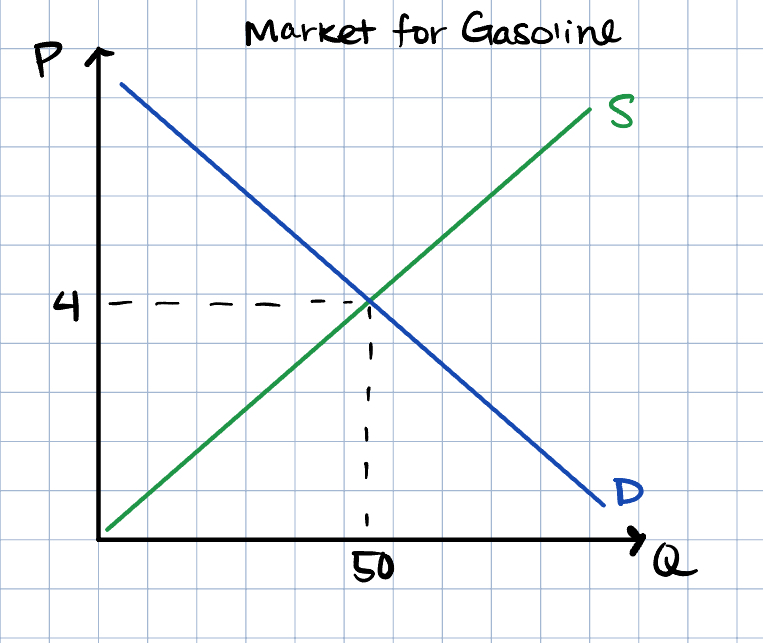
\includegraphics[width=.6\textwidth]{market_for_gas.png}
    \caption{Market for gasoline}
    \label{fig:market_for_gas}
\end{figure}

\begin{figure}[H]
    \centering
    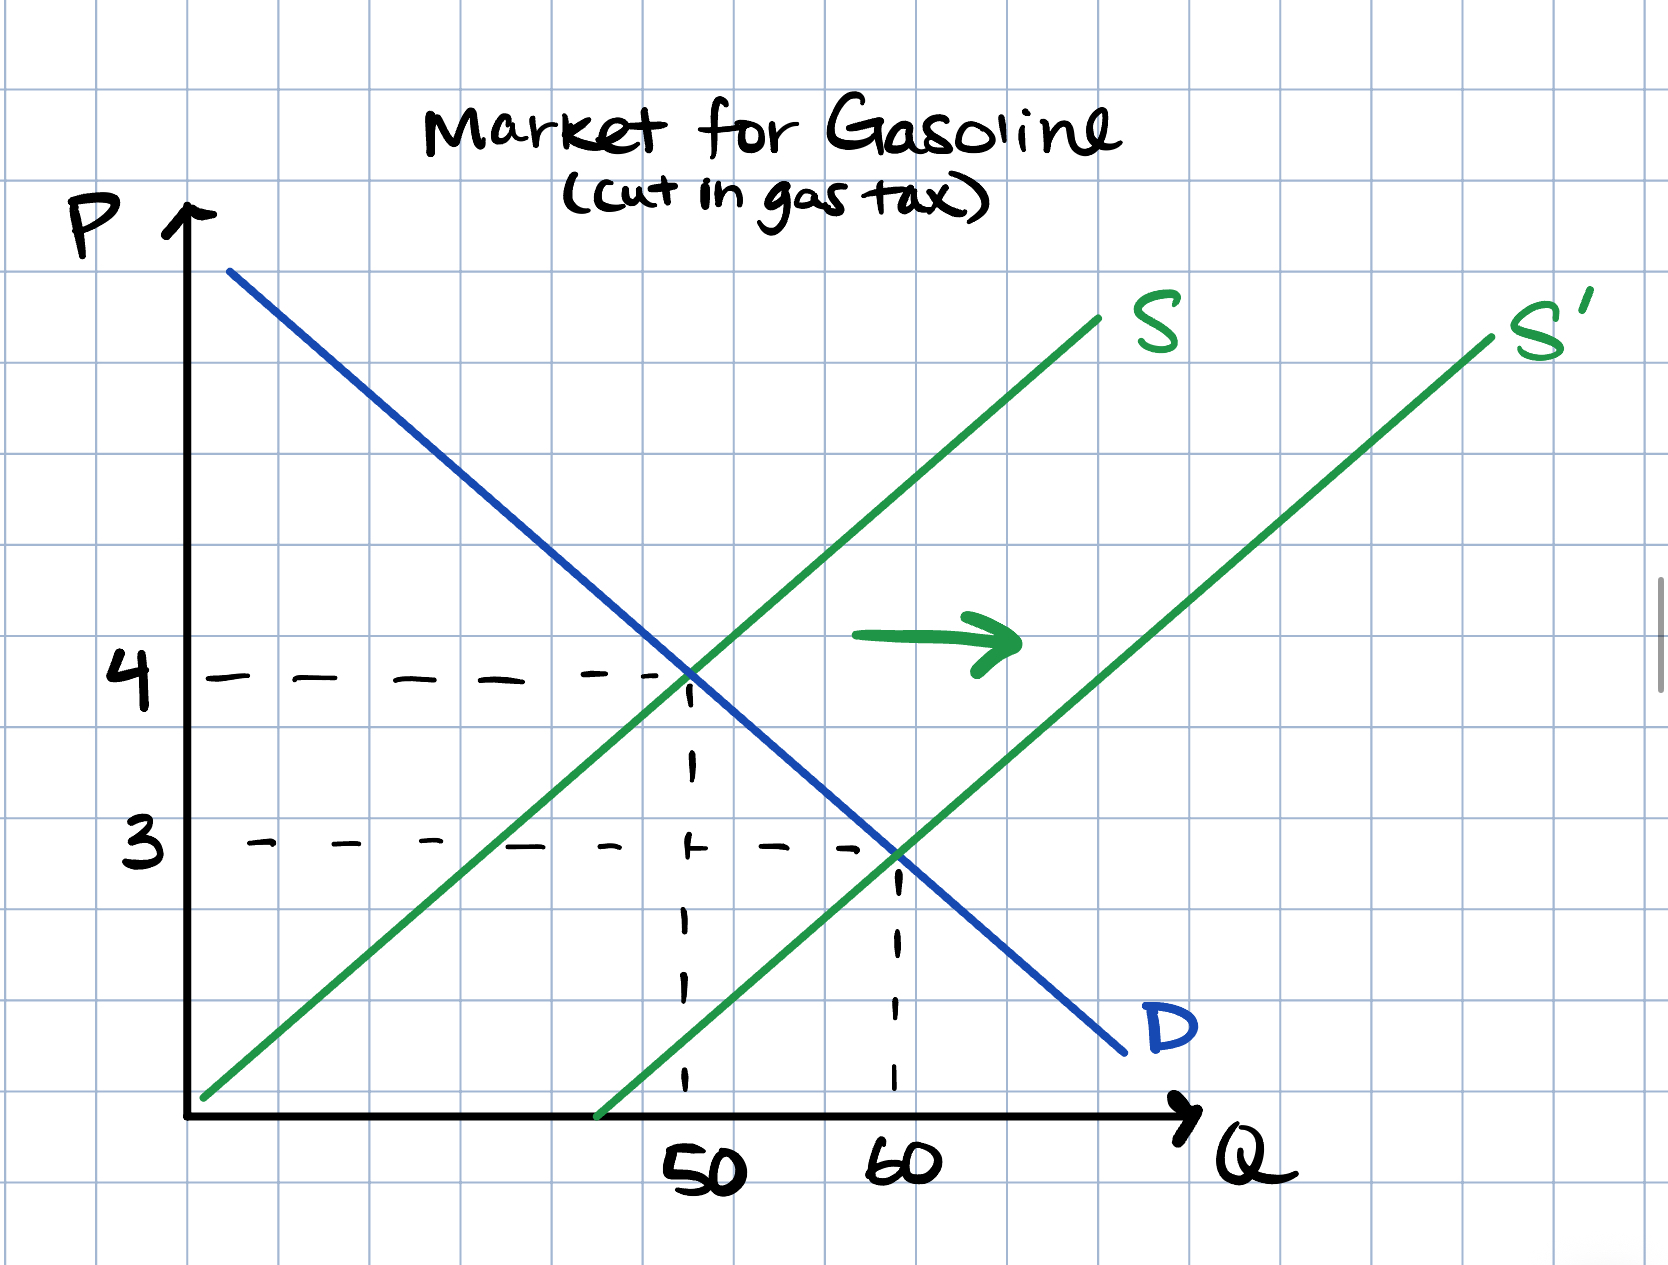
\includegraphics[width=.6\textwidth]{tax_cut.png}
    \caption{Effect of a tax cut}
    \label{fig:tax_cut}
\end{figure}

\item Increased fuel efficiency shifts our demand curve to the left; at any given price, we buy less gasoline than before, at a lower price. This will look like figure \ref{fig:increase_efficiency}.

\begin{figure}[H]
    \centering
    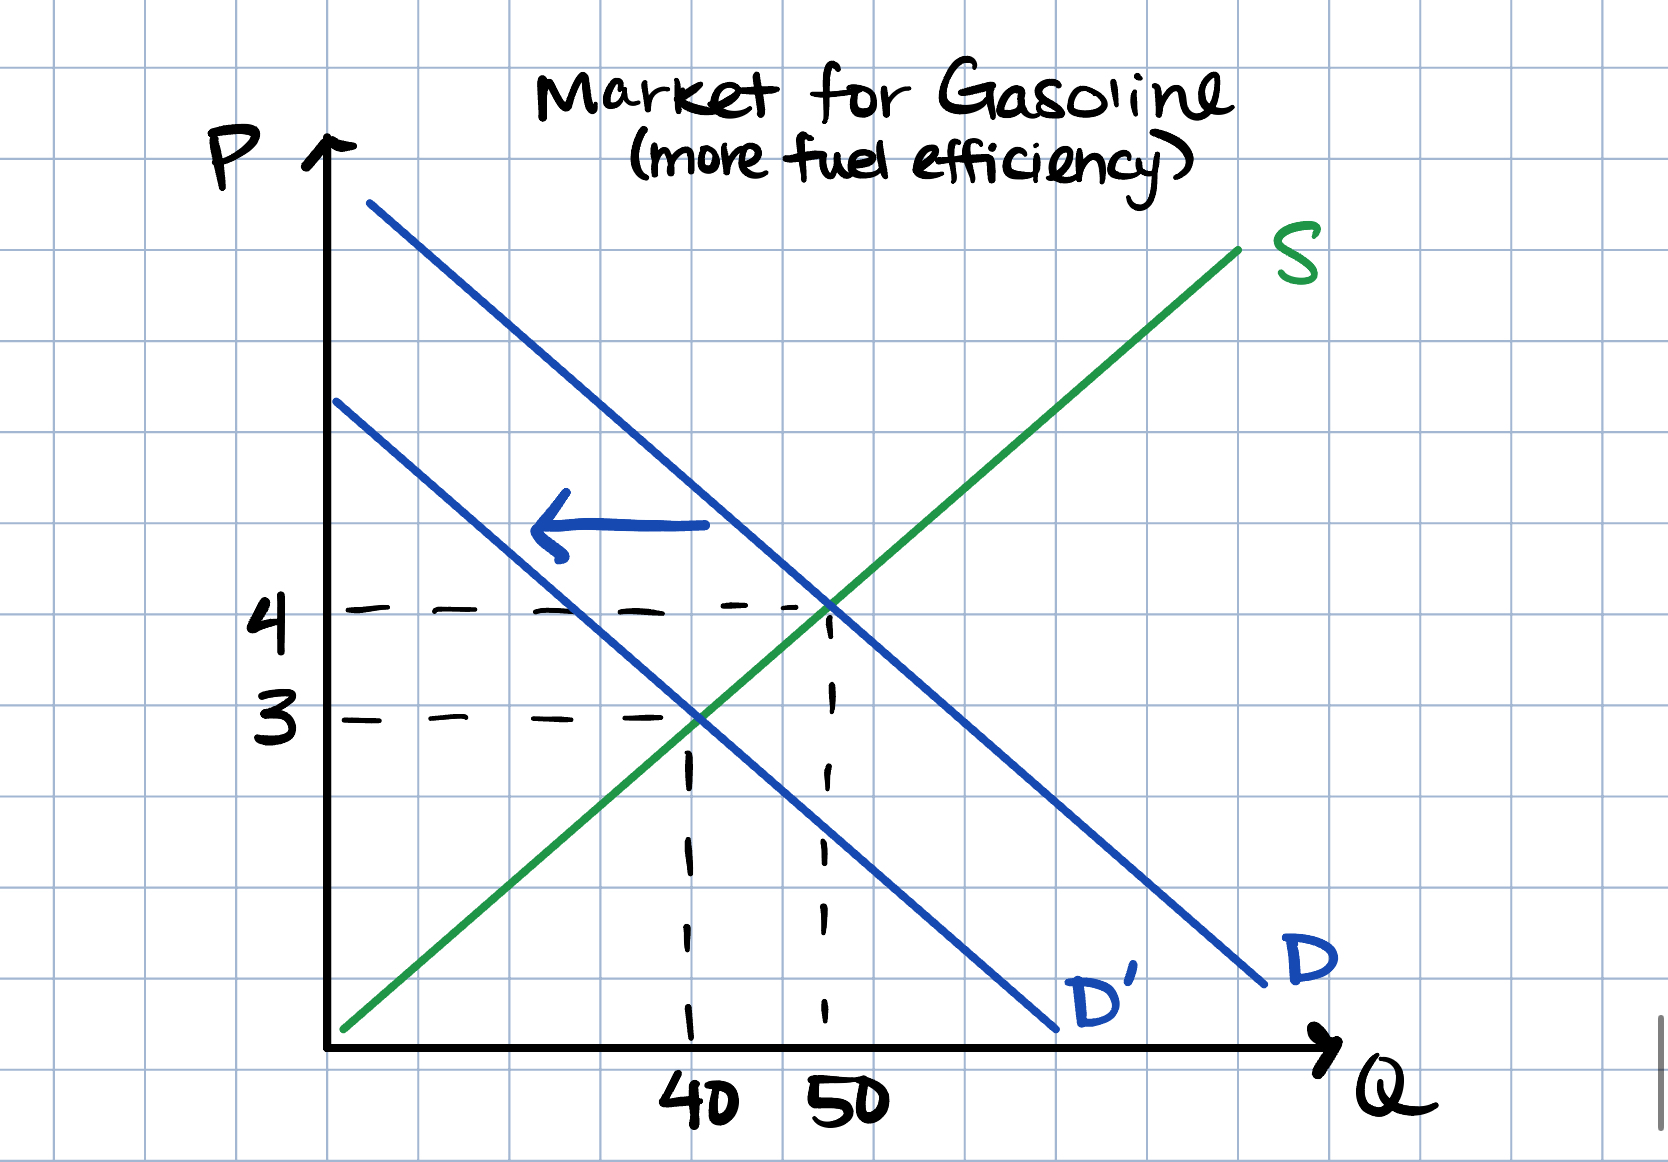
\includegraphics[width=.6\textwidth]{increase_efficiency.png}
    \caption{Increased fuel efficiency}
    \label{fig:increase_efficiency}
\end{figure}



\item From our previous answers, we know:
    \begin{itemize}
        \item The supply curve shifts to the right, so the price decreases and the quantity increases
        \item The demand curve shifts to the left, so the price decreases and the quantity decreases
    \end{itemize}

    So the equilibrium price must decrease, but the equilibrium quantity may increase or decrease; it depends on the magnitude of the two shifts! This means the new market might look like either figure \ref{fig:both_changes_1a} or figure \ref{fig:both_changes_1b}.

    \begin{figure}[H]
        \centering
        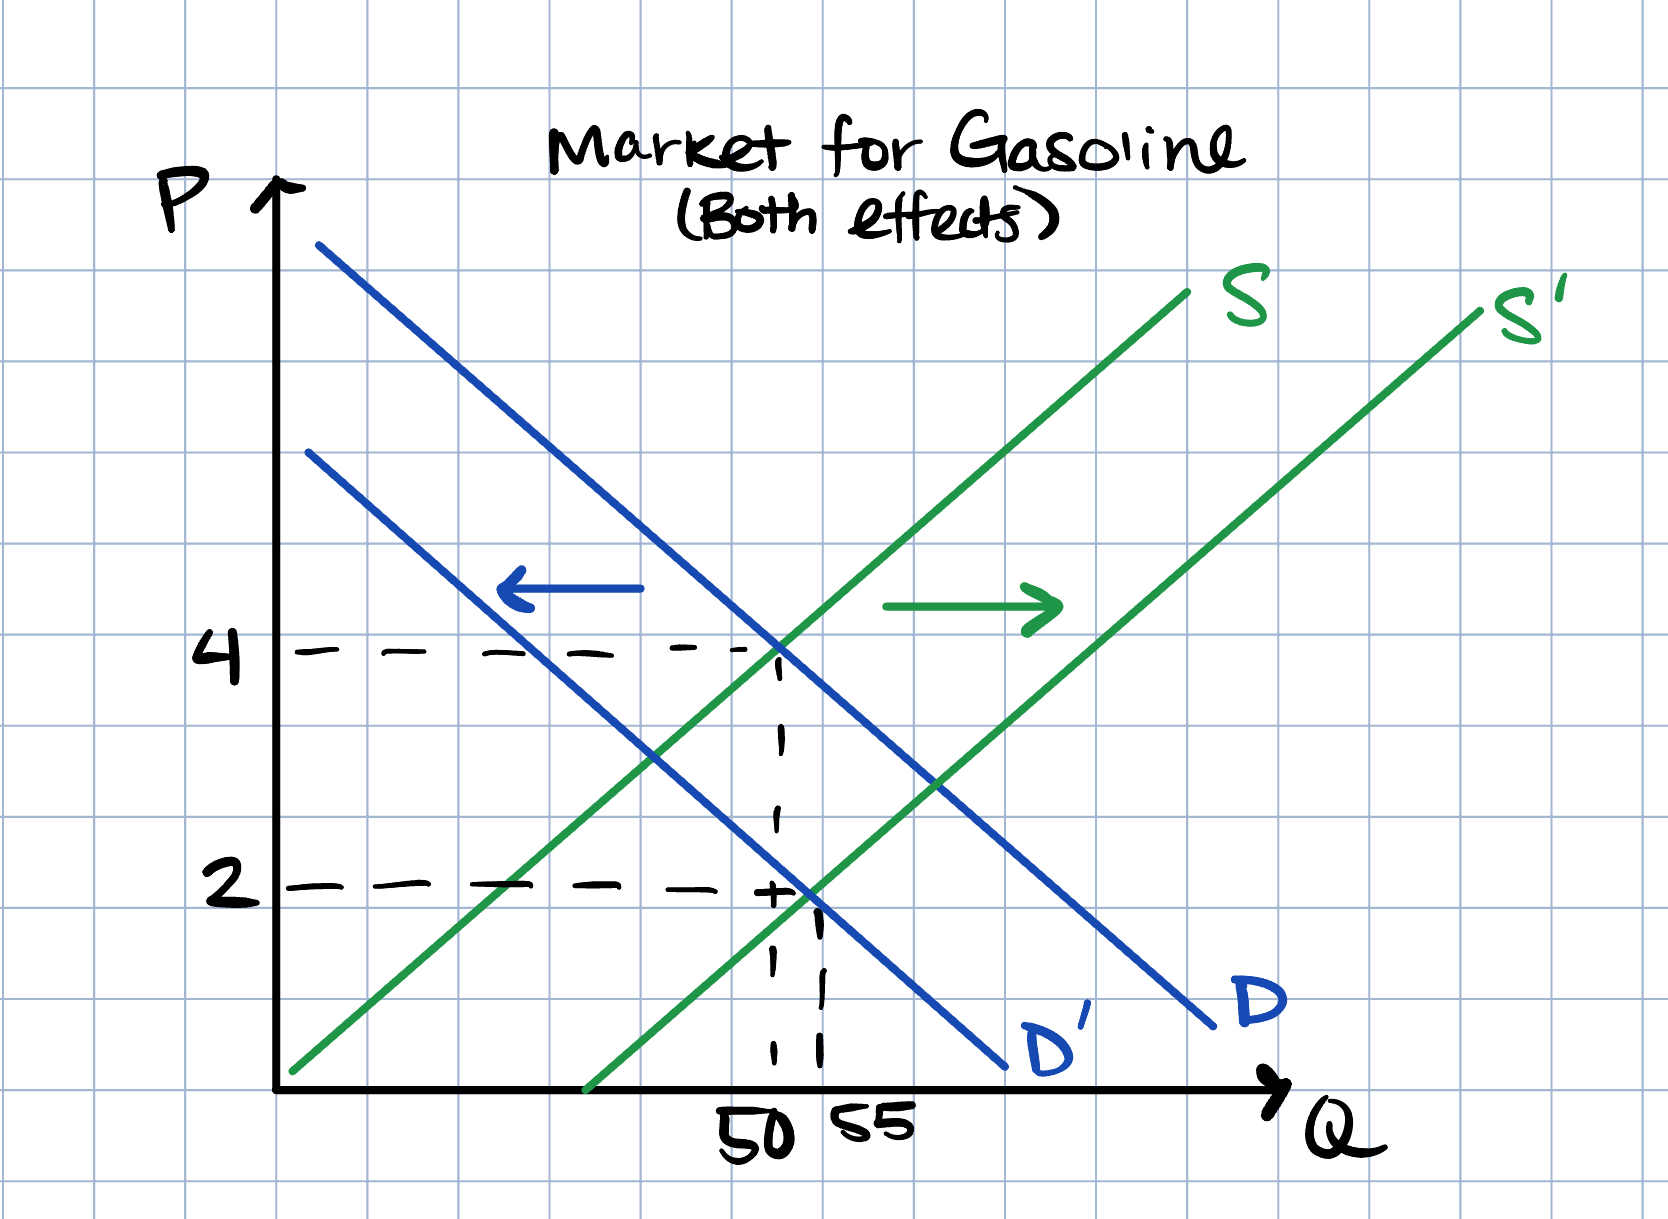
\includegraphics[width=.6\textwidth]{both_changes_1a.png}
        \caption{Tax cut and increased efficiency}
        \label{fig:both_changes_1a}
    \end{figure}

    \begin{figure}[H]
        \centering
        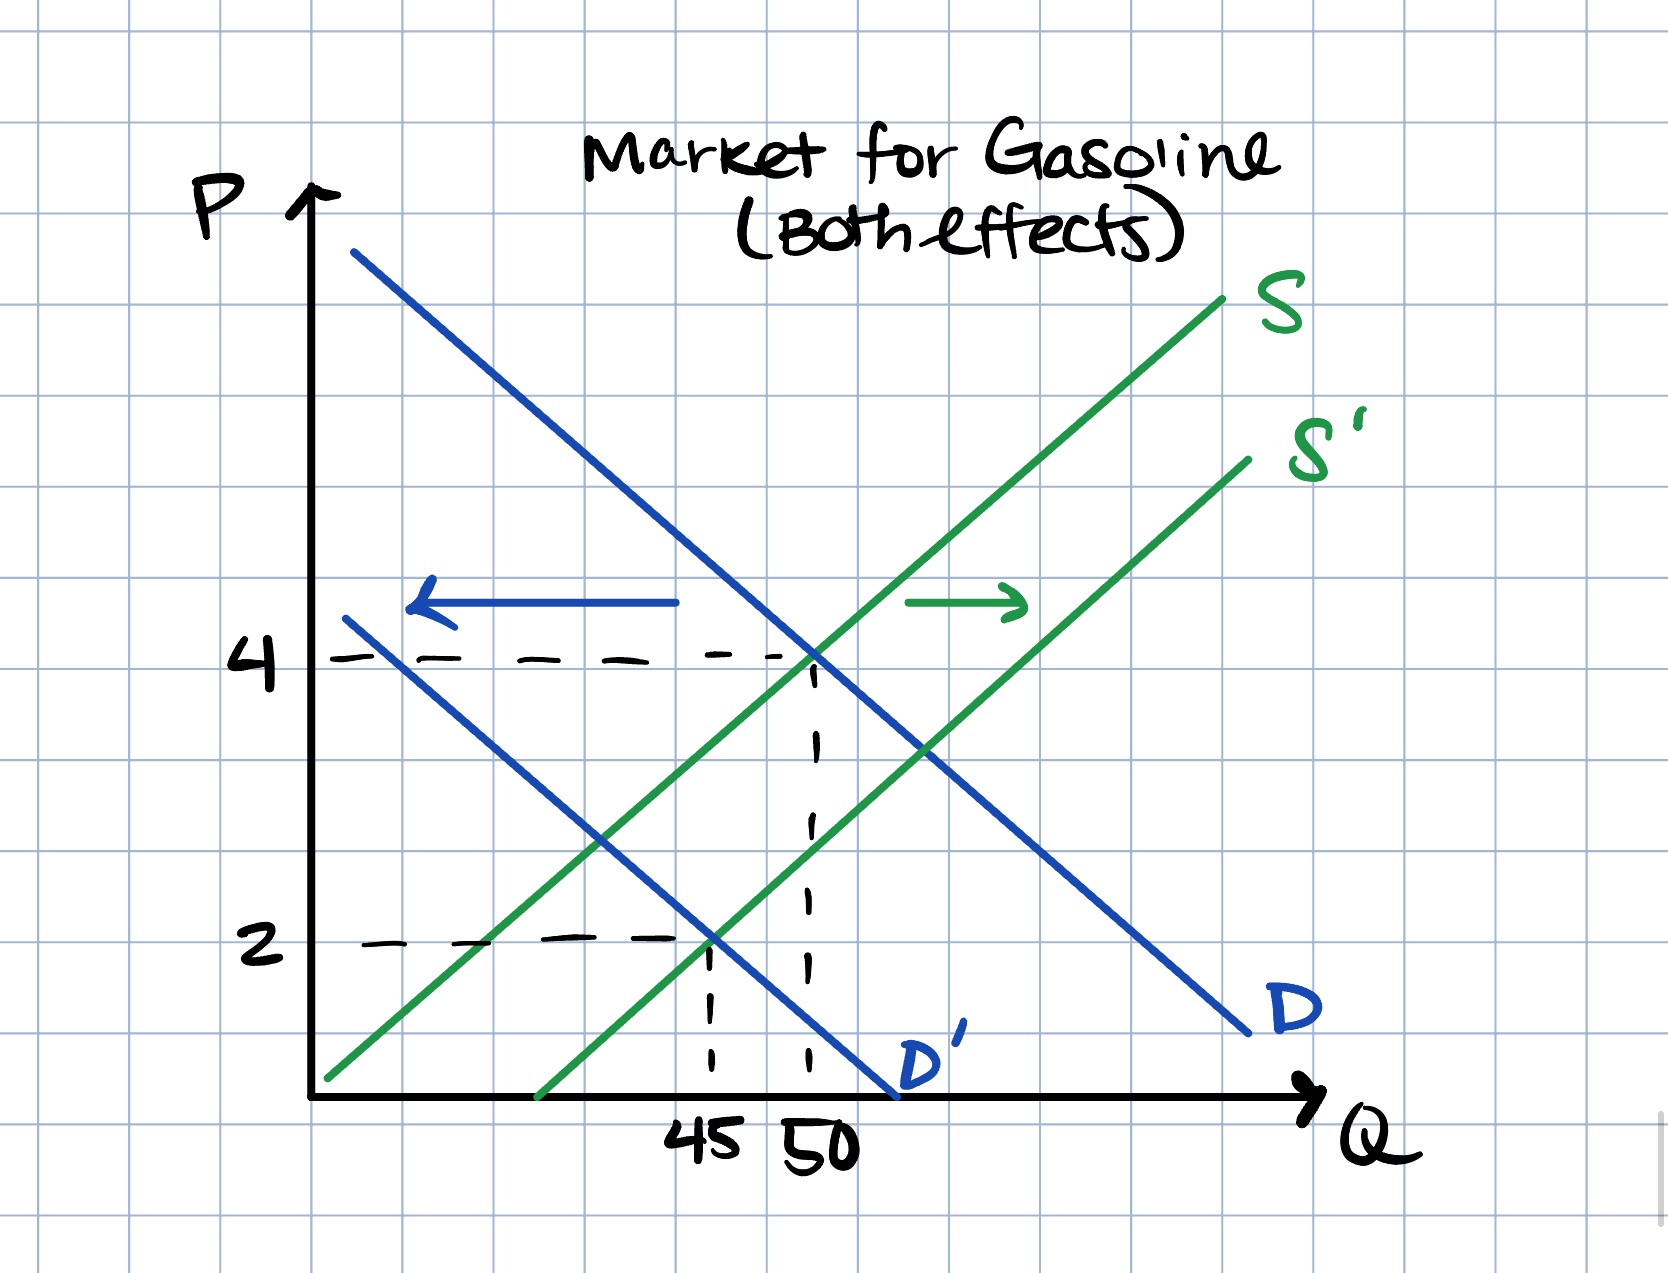
\includegraphics[width=.6\textwidth]{both_changes_1b.png}
        \caption{Tax cut and increased efficiency}
        \label{fig:both_changes_1b}
    \end{figure}

\item The decreased efficiency has, of course, the opposite impact as the increased efficiency, shown in figure \ref{fig:decrease_efficiency}. 

\begin{figure}[H]
    \centering
    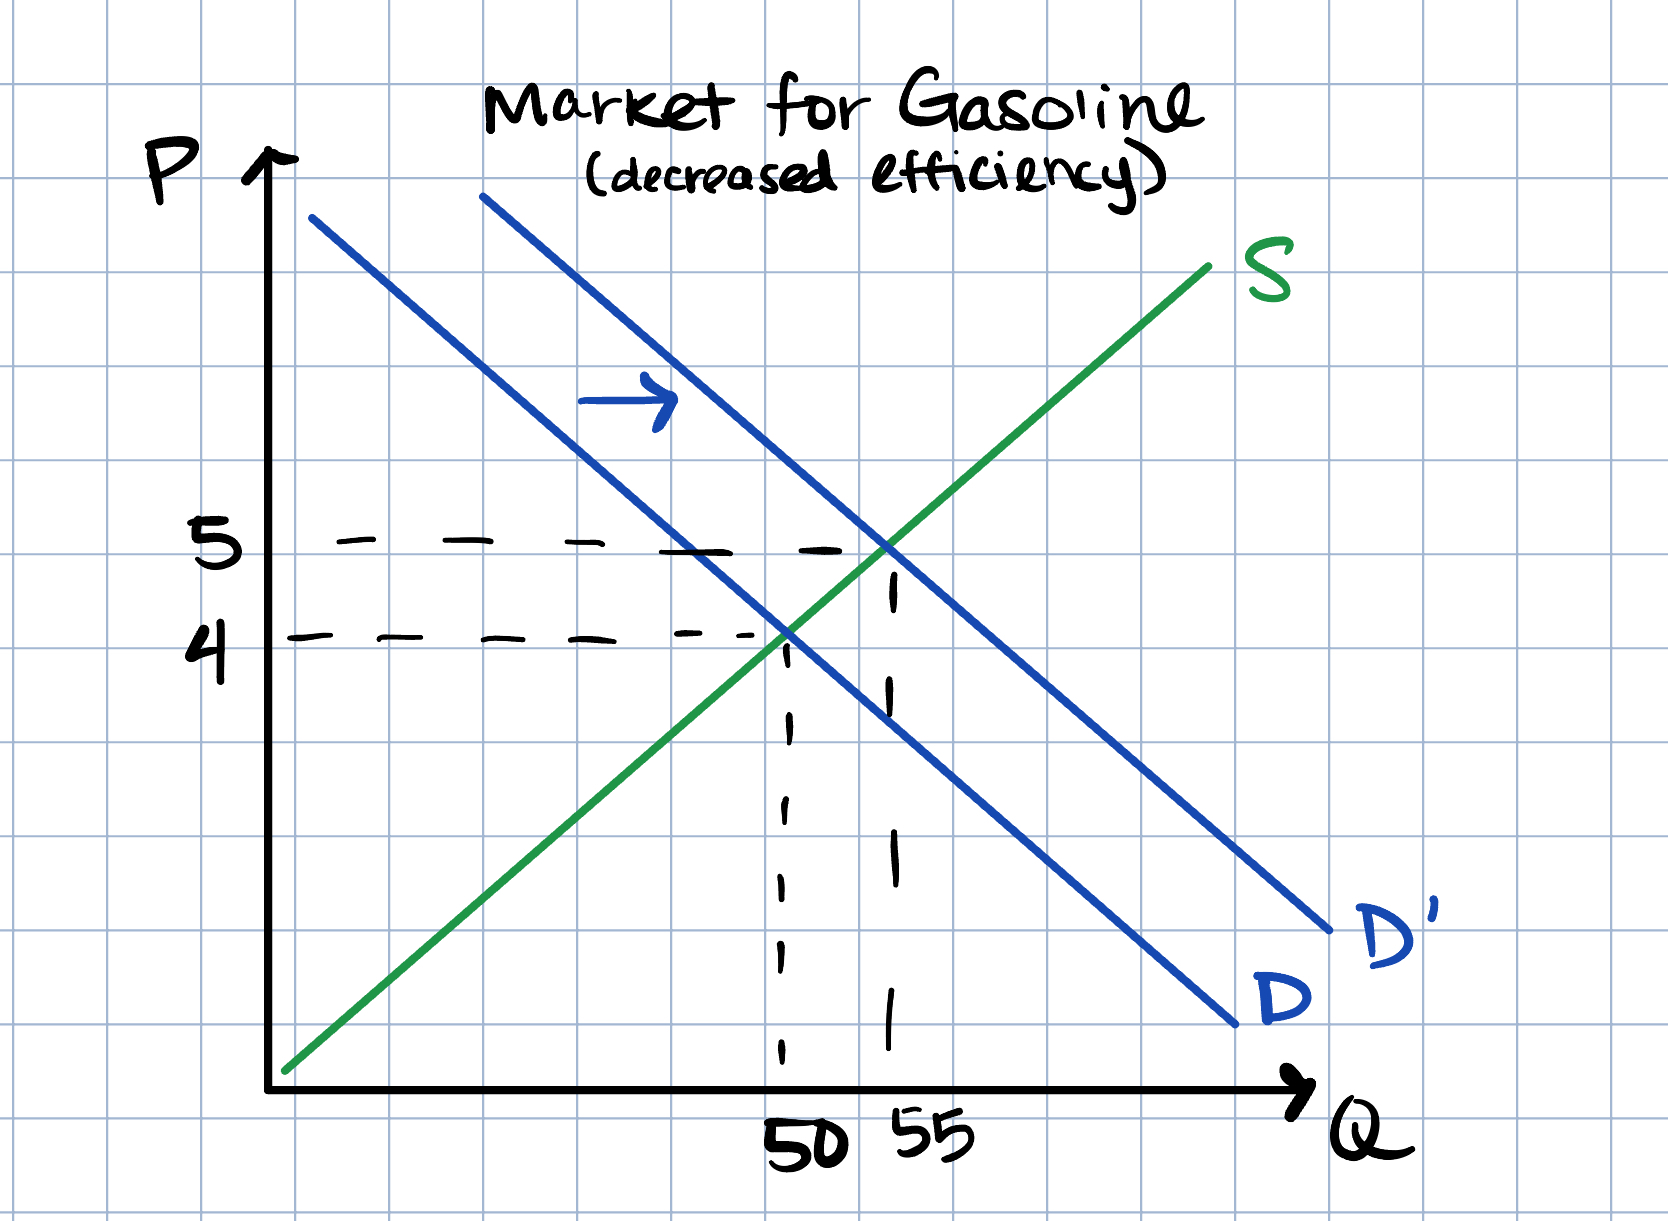
\includegraphics[width=.6\textwidth]{decrease_efficiency.png}
    \caption{Effect of decreased fuel efficiency}
    \label{fig:decrease_efficiency}
\end{figure}

As before, the new equilibrium is ambiguous, but in a slightly different way. We now have an increase in demand (higher quantity and higher price) and an increase in supply (higher quantity and lower price) so the equilibrium quantity must unambiguously increase, but the equilibrium price may increase or decrease depending on the magnitude of the shifts. These two possibilities are shown in figures \ref{fig:both_changes_2a} and \ref{fig:both_changes_2b}.

\begin{figure}[H]
    \centering
    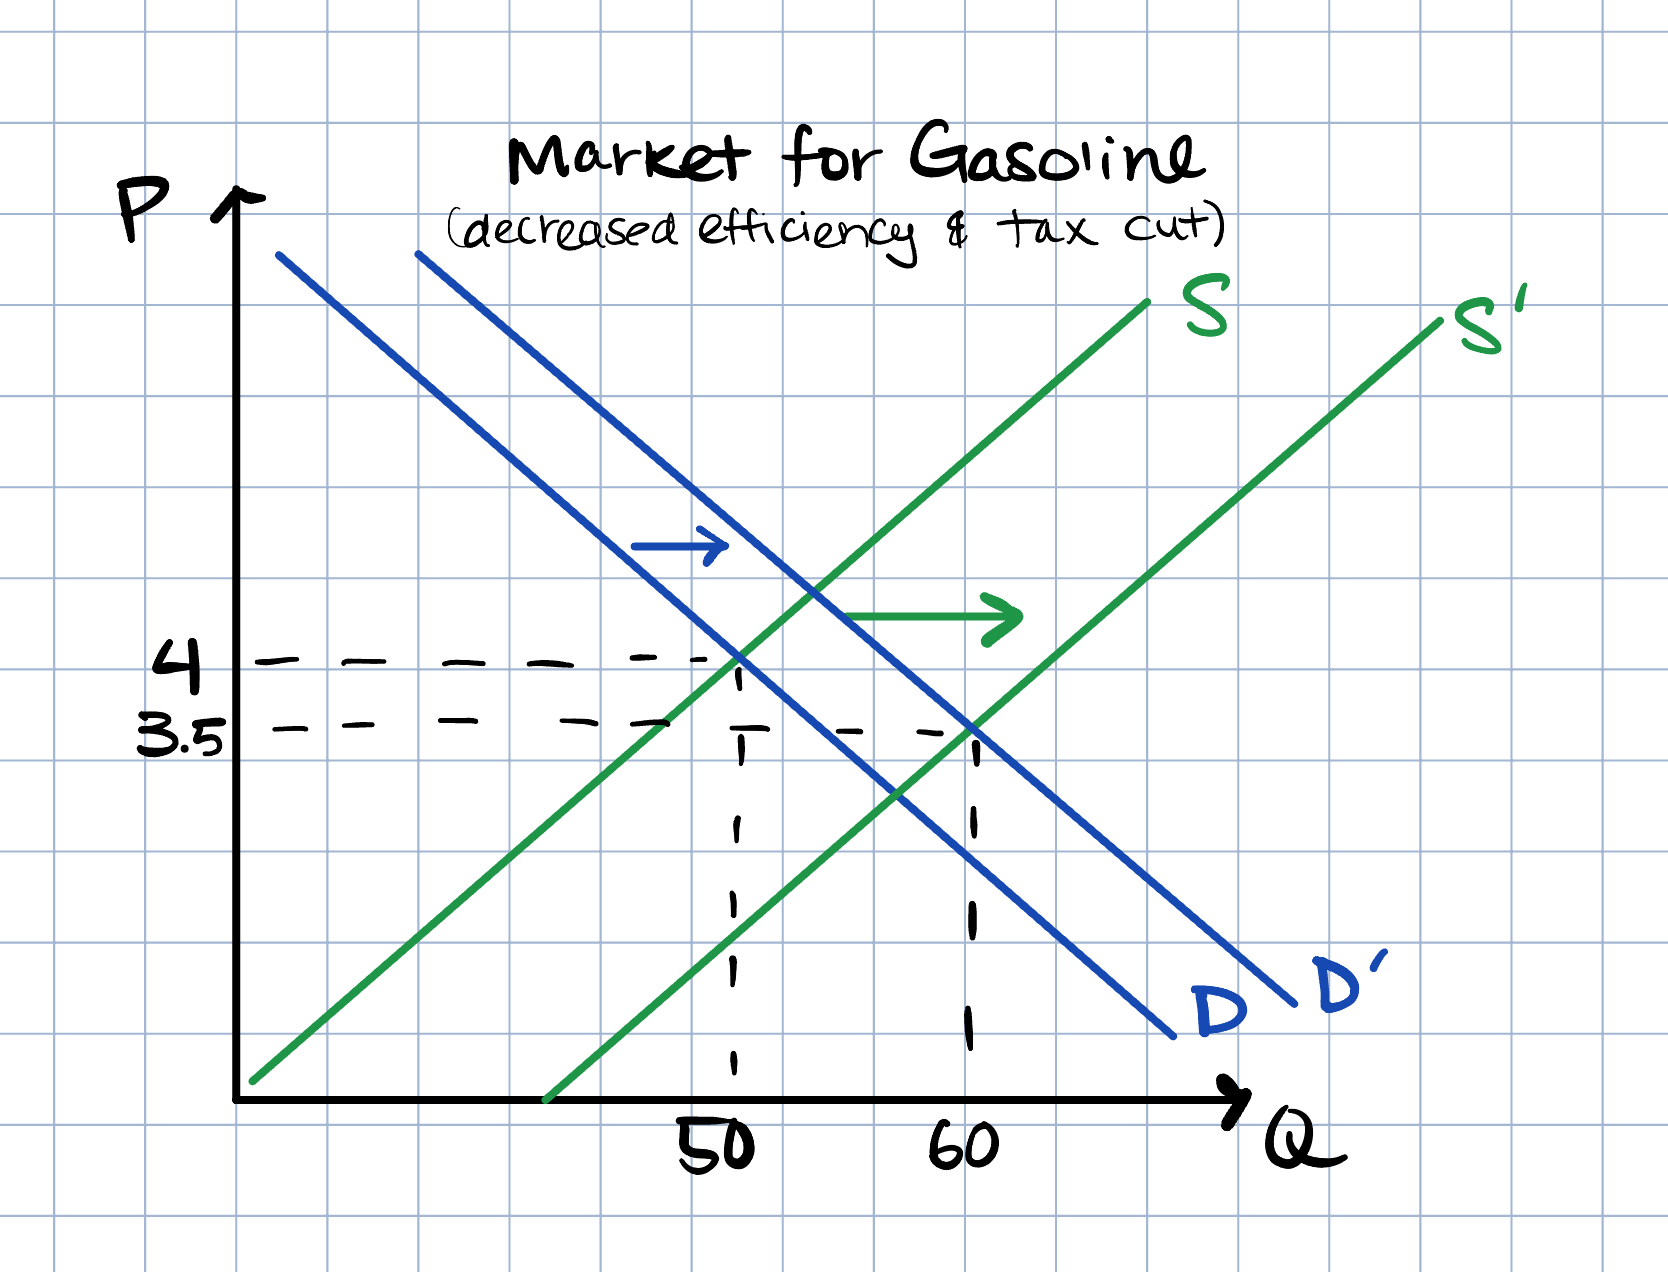
\includegraphics[width=.6\textwidth]{both_changes_2a.png}
    \caption{Tax cut and decreased efficiency}
    \label{fig:both_changes_2a}
\end{figure}

\begin{figure}[H]
    \centering
    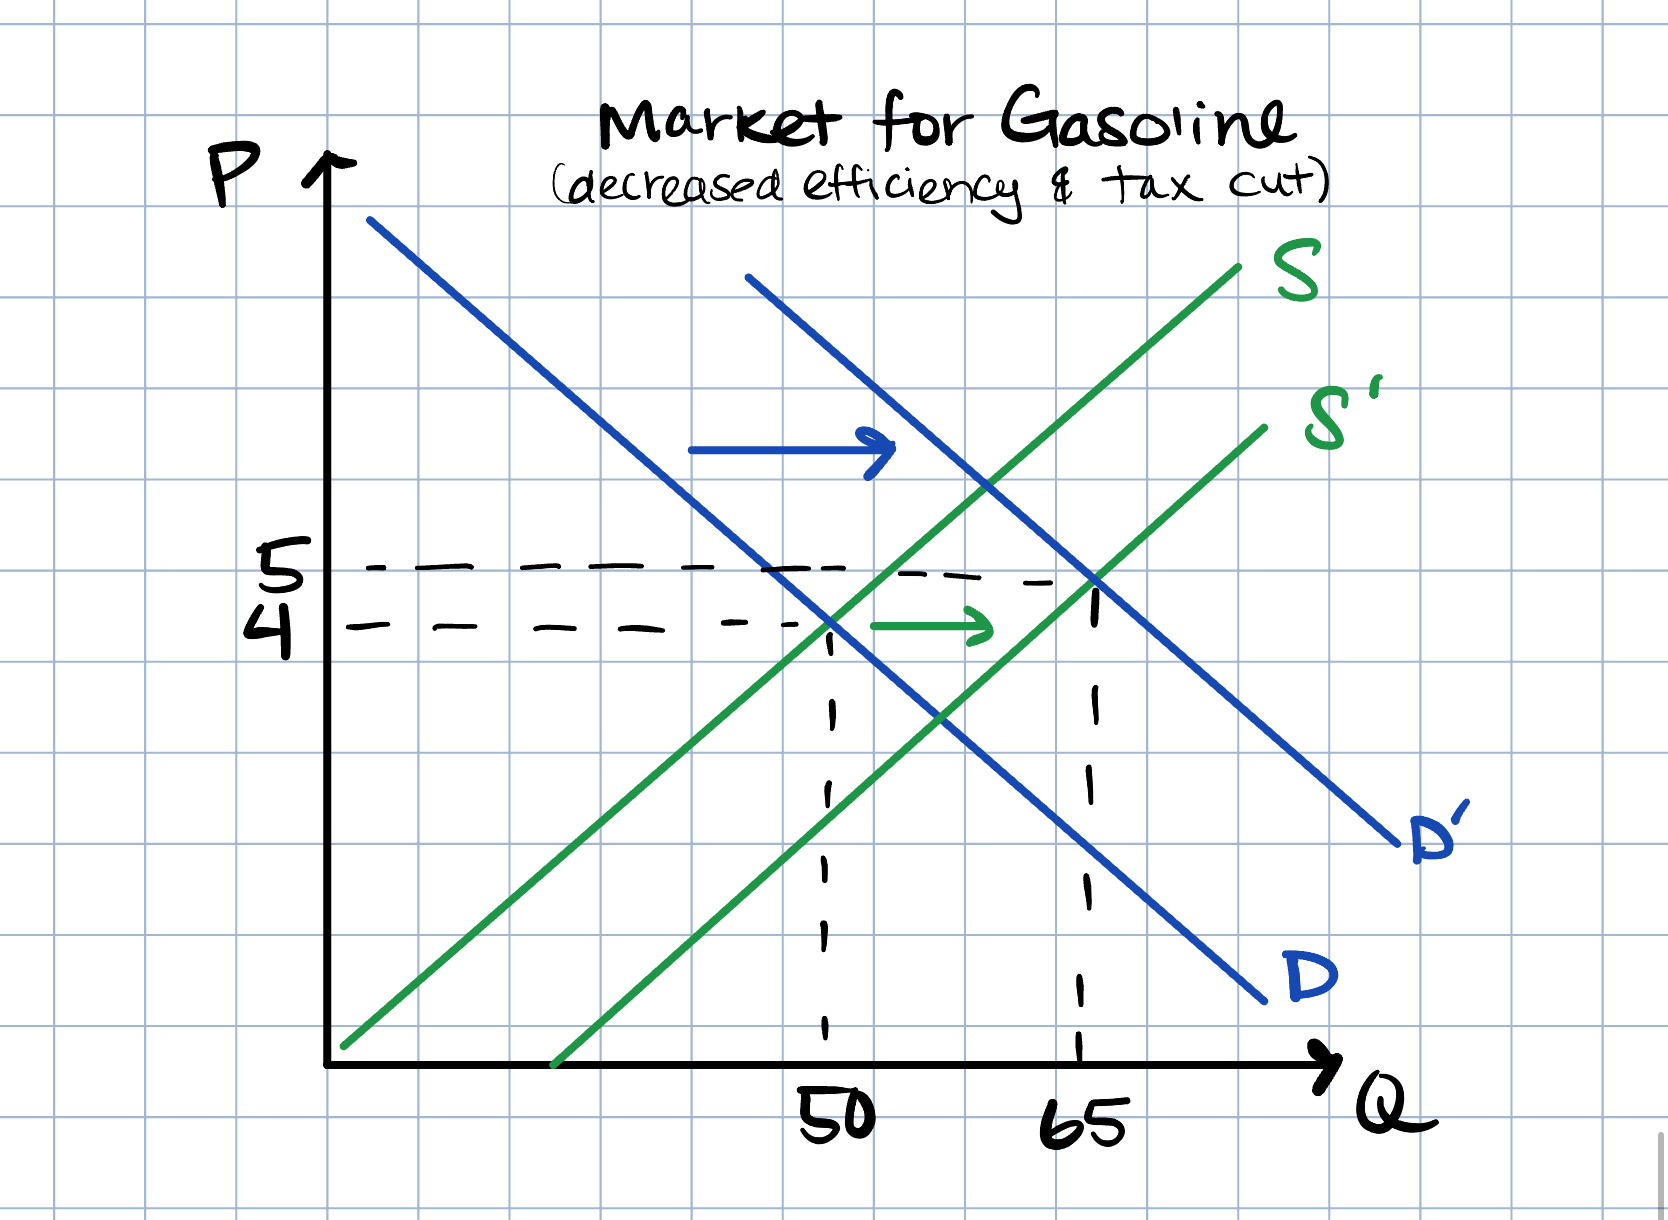
\includegraphics[width=.6\textwidth]{both_changes_2b.png}
    \caption{Tax cut and decreased efficiency}
    \label{fig:both_changes_2b}
\end{figure}
\end{enumerate}



\section*{Question 3}
In the last few years, the Orioles have gone from one of the worst teams in MLB to one of the best.

\begin{enumerate}
    \item Draw the supply and demand curves for Orioles tickets.
    \item Does the supply curve look like it did in the gasoline market?
    \item Will the team's improved record effect supply or demand, and why?
    \item What will happen to equilibrium price and quantity?
\end{enumerate}

\textbf{Answer: }

\begin{enumerate}

\item The market should look something like figure \ref{fig:orioles}.

\begin{figure}[H]
    \centering
    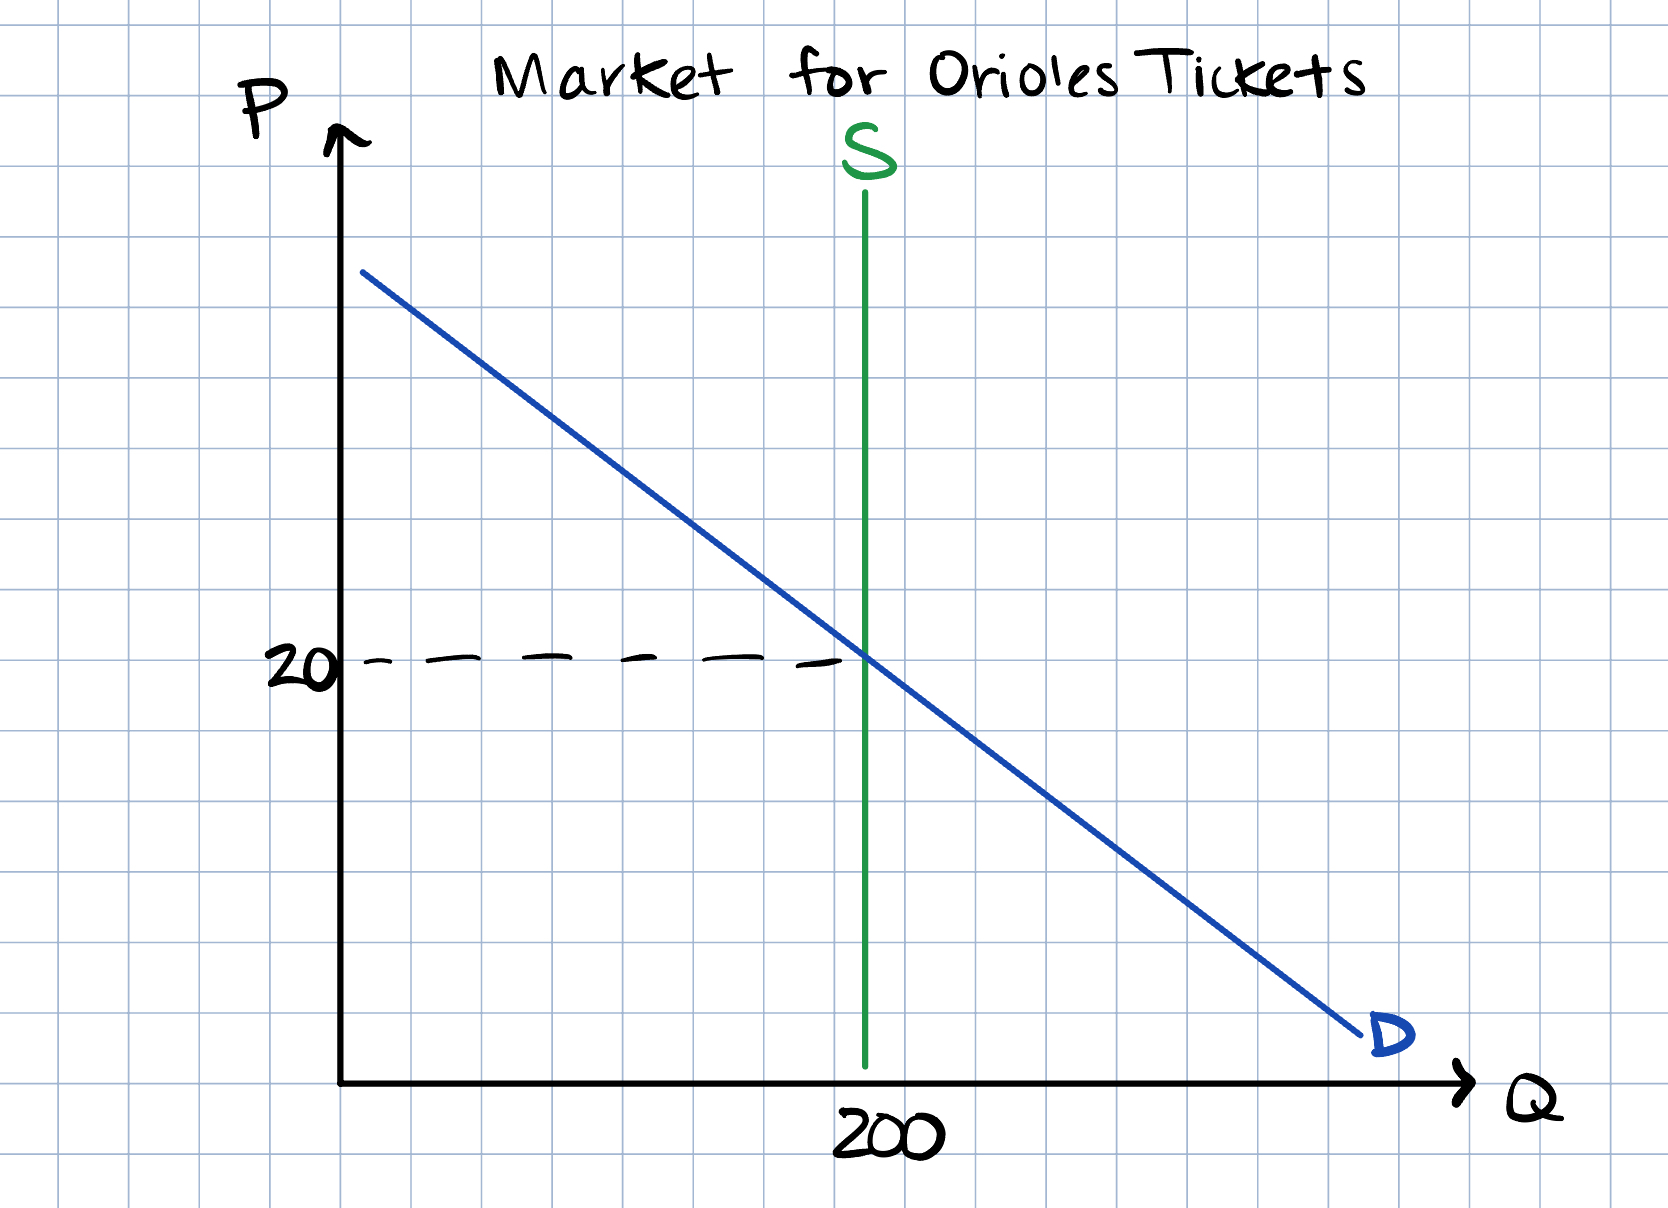
\includegraphics[width=.6\textwidth]{orioles.png}
    \caption{Market for Orioles tickets}
    \label{fig:orioles}
\end{figure}

\item What's important is that the supply curve is vertical. This is different from the market for gasoline, and from how we usually think about supply curves, and it reflects the reality that the owners of Camden Yards (the Orioles stadium) cannot increase or decrease supply. There are a certain number of seats in the stadium, no matter what the demand is.

\medskip

\item The team's improved record will effect the demand side only: at any given ticket price, more fans will want to go to the game. So the new equilibrium price will be unambiguously higher, while the quantity remains fixed. Figure~\ref{fig:orioles changes changes} depicts this change in the demand curve.

\item While this is a useful framework (the team being better really does mean that tickets have gotten more expensive!) it obviously ignores many ``real life'' issues. One objection might be that the team owners could build a new stadium with more seats. This is true, but can only happen in the long-run (such projects take years if not decades); also note that even with a larger stadium, the new supply curve will be vertical. If you get this kind of question on a test, you might make the distinction that \textit{in the short run} the supply curve is fixed, even though \textit{in the long run} the owners could theoretically build a new stadium.

\begin{figure}[H]
    \centering
    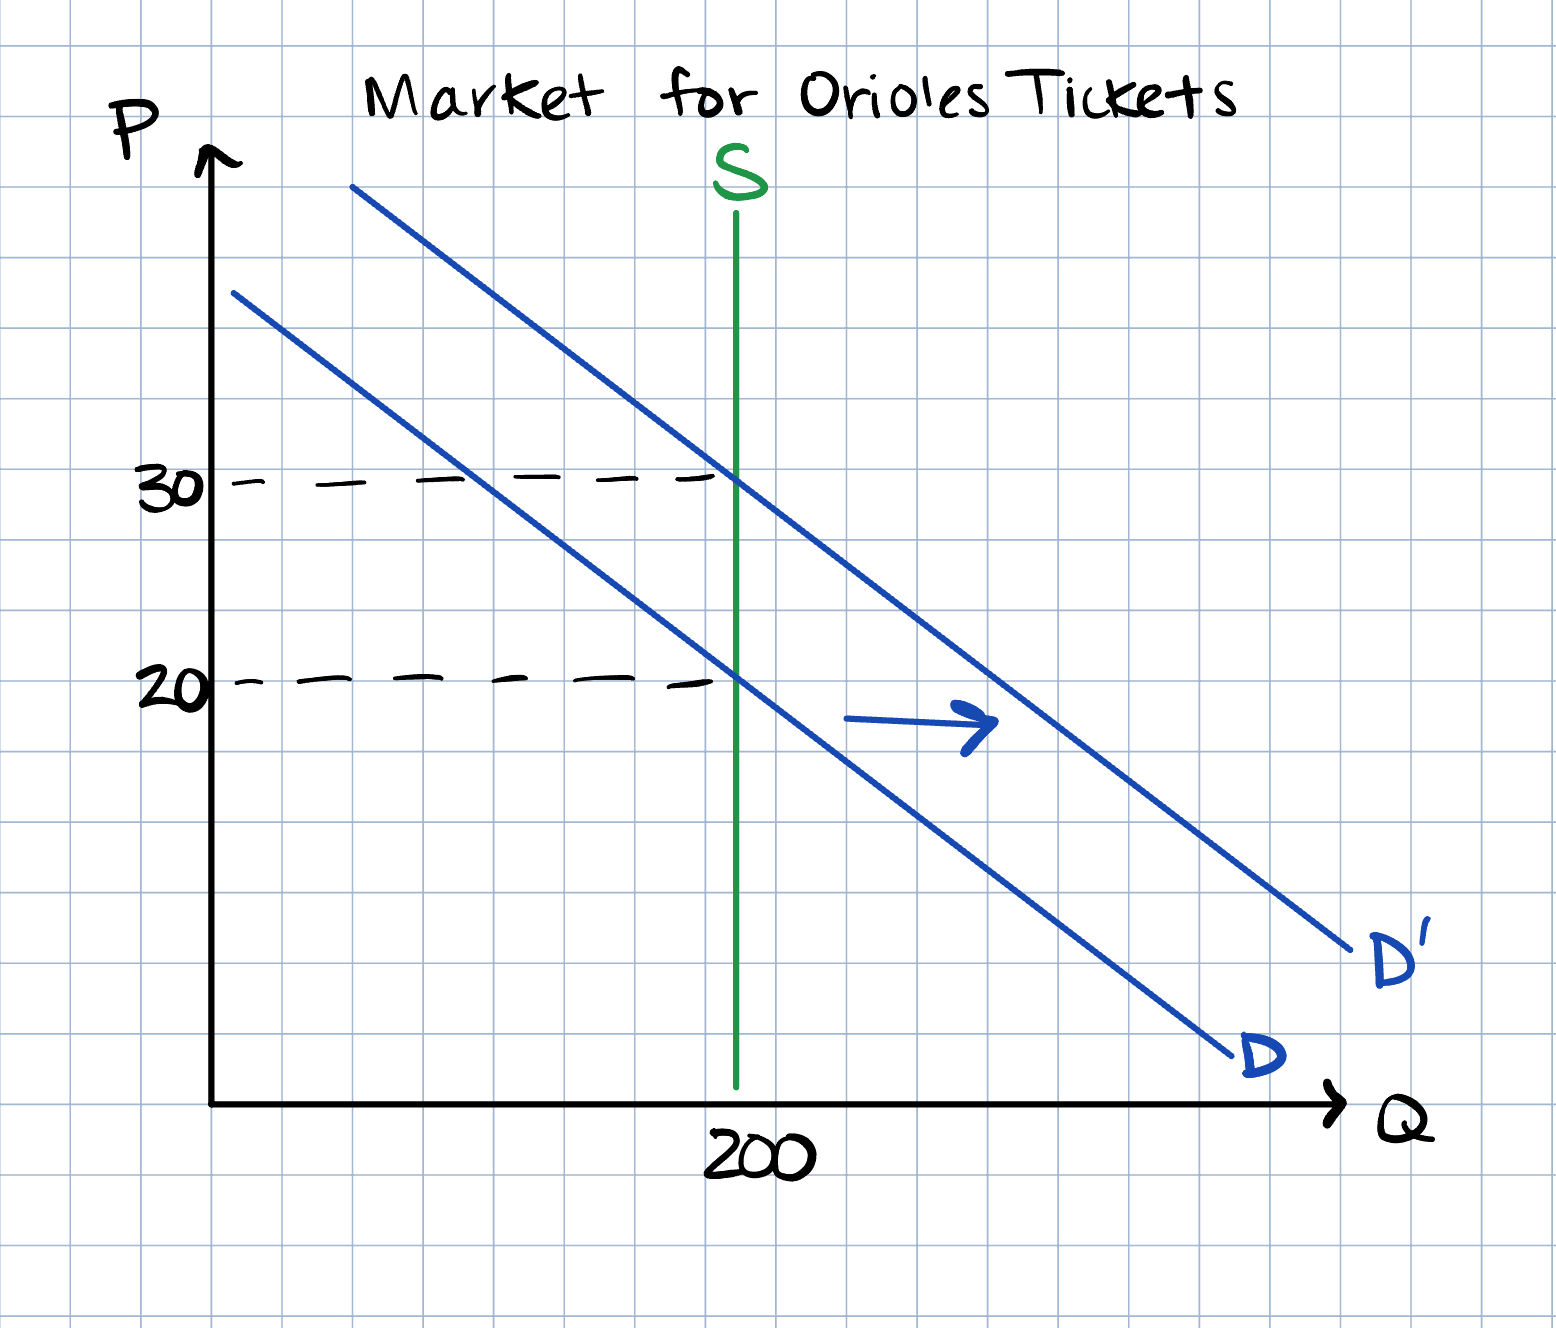
\includegraphics[width=.6\textwidth]{orioles_changes.png}
    \caption{Shift in demand for Orioles tickets}
    \label{fig:orioles changes}
\end{figure}

\end{enumerate}



\end{document}
